\documentclass{article}

% these packages let you do math
\usepackage{amsmath}
\usepackage{amssymb}

% we need these packages for fancy R tables
\usepackage{booktabs}
\usepackage{float}
\usepackage{colortbl}
\usepackage{xcolor}

% these packages play with the spacing/margins of the document. Uncomment the commands on lines 16 and 17 to see what they do.
\usepackage{a4wide}
\usepackage{setspace}
\usepackage{geometry}
\usepackage{parskip}
%\doublespacing
%\geometry{margin=1.5in}

% this package helps us with including images. Setting the graphics path makes it easier to refer to things in the \includegraphics command.
\usepackage{graphicx}
\graphicspath{ {../figures/} }

% make some hyperlinks using the \href command
\usepackage{hyperref}
\hypersetup{
    colorlinks=true,
    linkcolor=black,
    urlcolor=blue
}

% set the author, title, and date of the document. \maketitle adds it to the document.
\author{David Scolari}
\title{My Paper on NLSY97 Incarceration Data}
\date{Sping 2022}

\begin{document}
\maketitle

\section{The First Section}

\begin{table}[H]

\caption{\label{tab:tab:summarystats}Per Person Incarceration Days}
\centering
\begin{tabular}[t]{lrr}
\toprule
Race & Female & Male\\
\midrule
\cellcolor{gray!6}{Black} & \cellcolor{gray!6}{0.6426056} & \cellcolor{gray!6}{14.833333}\\
Hispanic & 0.9064570 & 4.804340\\
\cellcolor{gray!6}{Non-Black / Non-Hispanic} & \cellcolor{gray!6}{0.5876265} & \cellcolor{gray!6}{3.344241}\\
\bottomrule
\end{tabular}
\end{table}


Table 1 shows per person incarceration days for each racial group in 2002. Mixed race is omitted from the analysis due to limited sample size. The table shows that for each racial group, males spend more days incarcerated per individual than females. However, the increase in incarceration time for males compared to females is several times larger for black males than other other race.

This fact is highlighted by Figure 1, which shows the male to female ratio of days incarcerated for the three racial groups of interest. We see again that black males spent nearly 30 days incarcerated for every 1 day a black female spent incarcerated.  


\begin{figure}[H]
    \begin{center}
        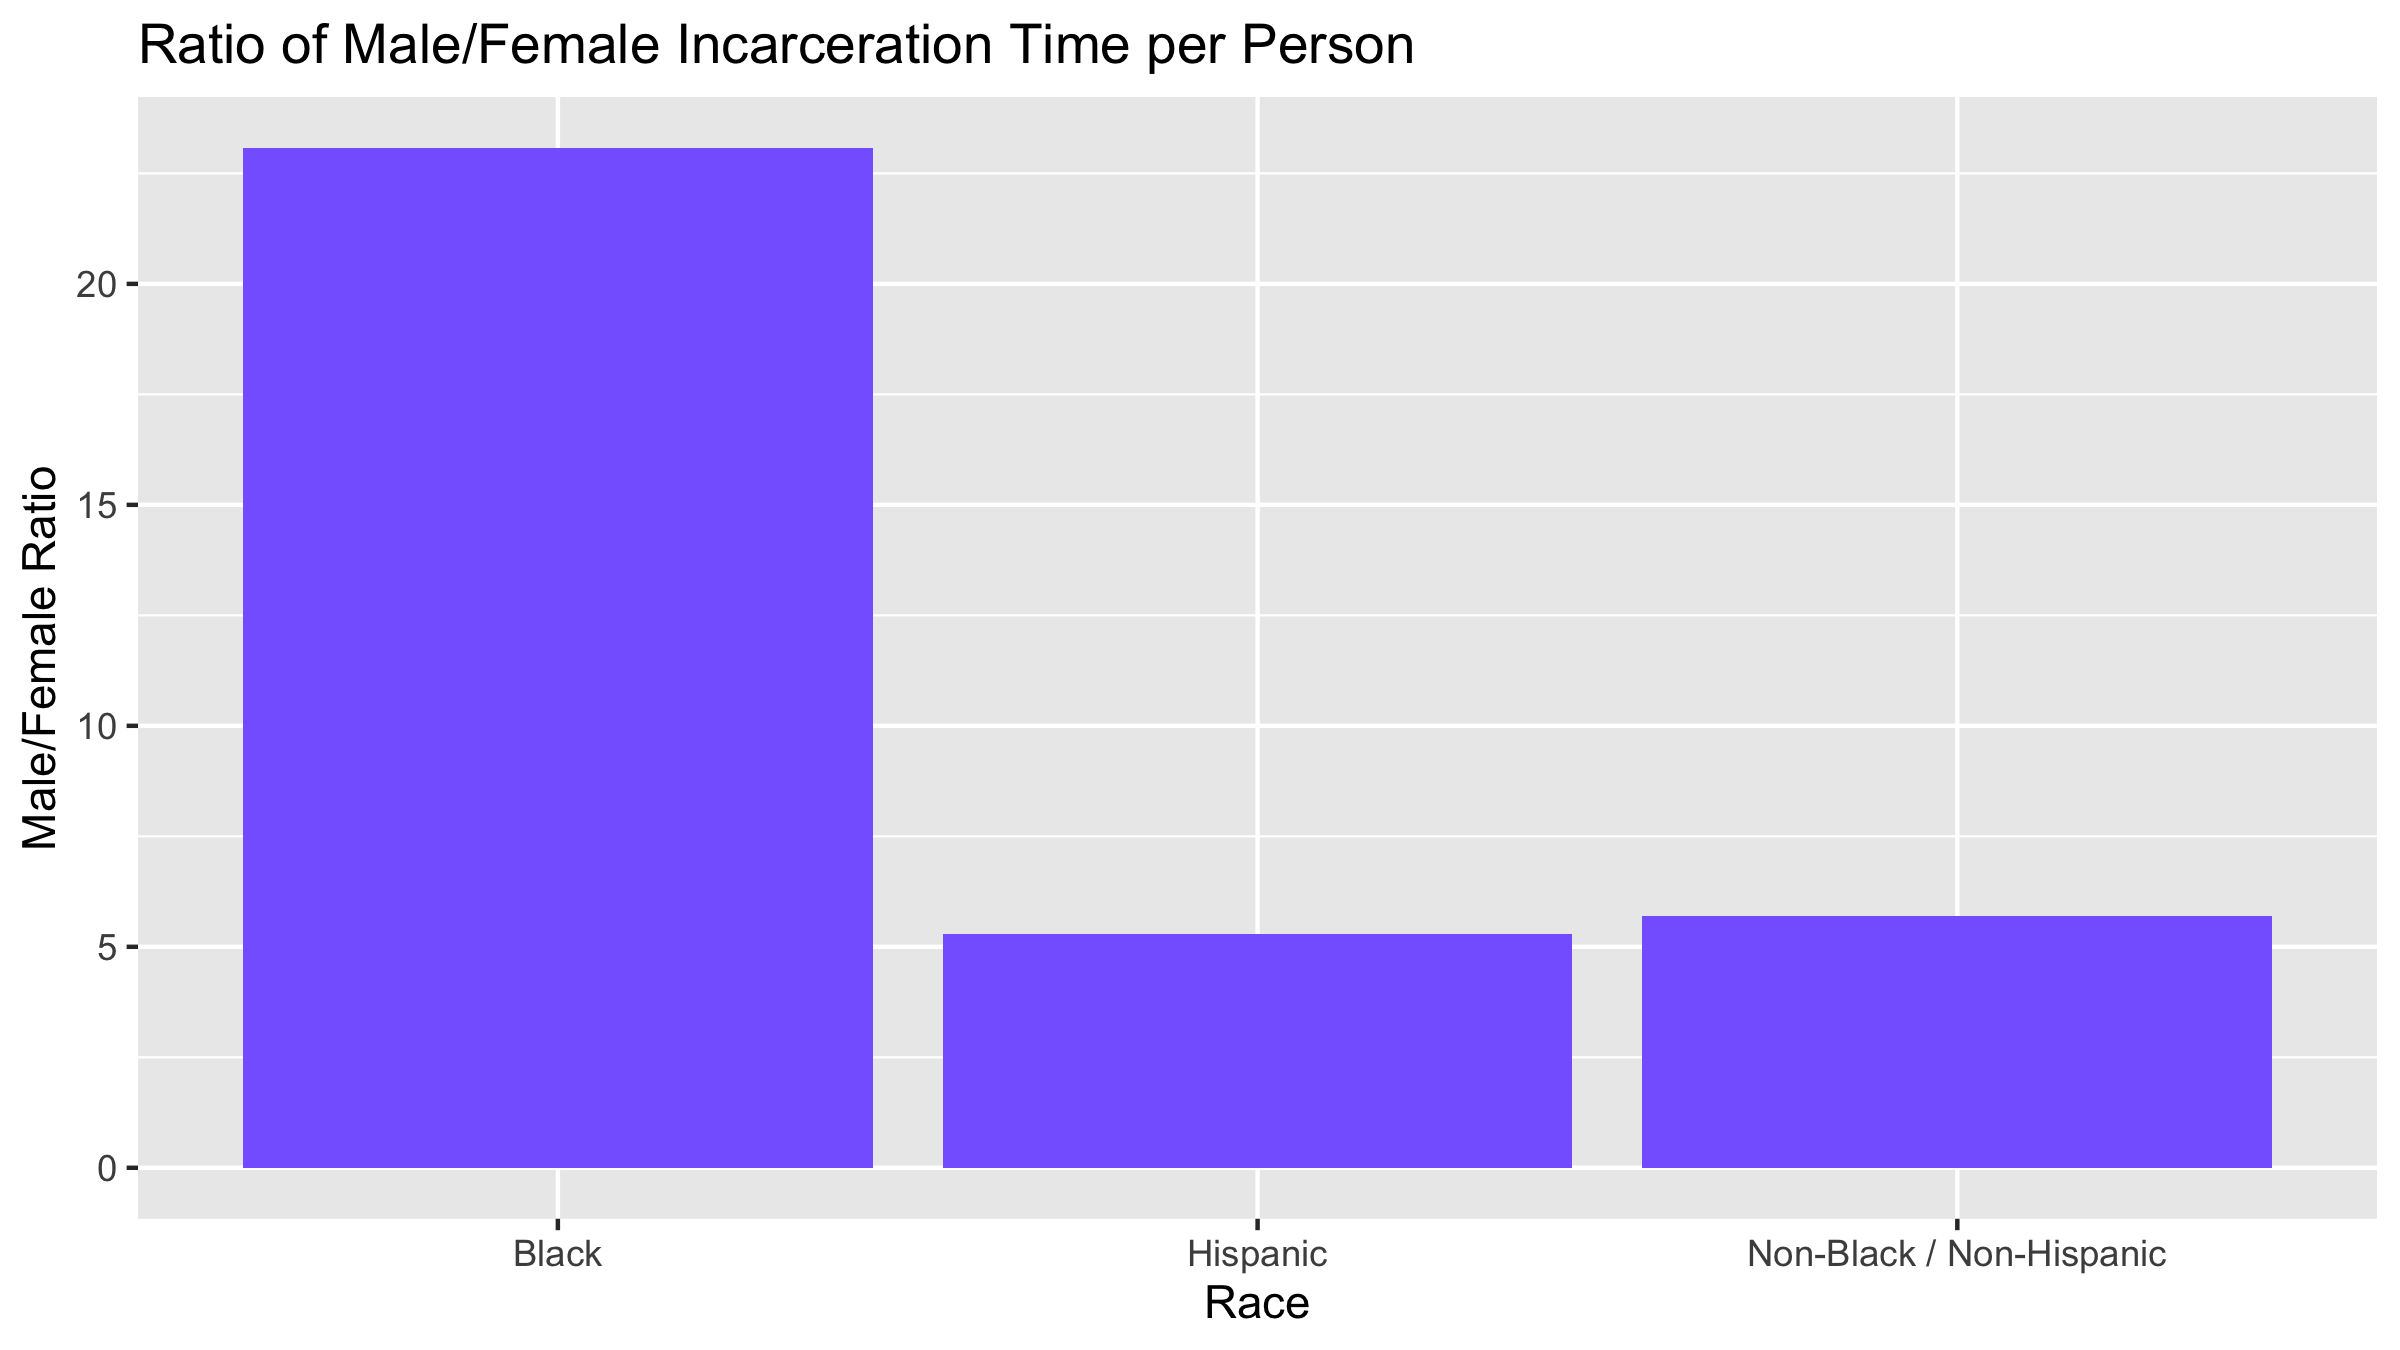
\includegraphics[width=.85\textwidth]{../figures/inc_bar.png}
    \end{center}
    \caption{Mean Number of Arrests in 2002 by Race and Gender (this is the LaTeX caption, not the ggplot title)}
    \label{fig:graph}
\end{figure}




% Table created by stargazer v.5.2.2 by Marek Hlavac, Harvard University. E-mail: hlavac at fas.harvard.edu
% Date and time: Thu, Feb 17, 2022 - 18:17:42
\begin{table}[!htbp] \centering 
  \caption{Regression Output. Omitted category is Black Females.} 
  \label{tab:regression} 
\begin{tabular}{@{\extracolsep{5pt}}lc} 
\\[-1.8ex]\hline 
\hline \\[-1.8ex] 
 & \multicolumn{1}{c}{\textit{Dependent variable:}} \\ 
\cline{2-2} 
\\[-1.8ex] & Per Person Incarceration Time in 2002 (days) \\ 
\hline \\[-1.8ex] 
 Hispanic & $-$4.823$^{***}$ \\ 
  & (1.169) \\ 
  & \\ 
 Mixed Race (Non-Hispanic) & $-$5.300$^{**}$ \\ 
  & (2.527) \\ 
  & \\ 
 Non-Black / Non-Hispanic & $-$5.737$^{***}$ \\ 
  & (1.053) \\ 
  & \\ 
 Male & 5.894$^{***}$ \\ 
  & (0.671) \\ 
  & \\ 
 Constant & 4.715$^{***}$ \\ 
  & (0.777) \\ 
  & \\ 
\hline \\[-1.8ex] 
Observations & 8,621 \\ 
R$^{2}$ & 0.015 \\ 
Adjusted R$^{2}$ & 0.014 \\ 
Residual Std. Error & 30.997 (df = 8616) \\ 
F Statistic & 32.033$^{***}$ (df = 4; 8616) \\ 
\hline 
\hline \\[-1.8ex] 
\textit{Note:}  & \multicolumn{1}{r}{$^{*}$p$<$0.1; $^{**}$p$<$0.05; $^{***}$p$<$0.01} \\ 
\end{tabular} 
\end{table} 


\end{document}